\documentclass[11pt,a4paper]{article}

\usepackage[margin=2.2cm]{geometry}
\usepackage{amsmath,amssymb}
\usepackage{booktabs}
\usepackage{array}
\usepackage{xcolor}
\usepackage{tikz}
\usepackage{fancyvrb}
\usepackage[hidelinks]{hyperref}
\usetikzlibrary{positioning,arrows.meta,fit,calc,shapes.geometric,backgrounds}

\definecolor{idxblue}{HTML}{2F6FED}
\definecolor{lakeblue}{HTML}{377ADD}
\definecolor{metagold}{HTML}{E0A030}
\definecolor{nasared}{HTML}{C0504D}
\definecolor{soft}{HTML}{6B7A8D}
\definecolor{panel}{HTML}{F2F5F9}
\definecolor{cellA}{HTML}{4C9A6B}
\definecolor{cellB}{HTML}{8A63C0}

\newcommand{\code}[1]{\texttt{\small #1}}
\newcommand{\col}[1]{\texttt{\footnotesize #1}}

\tikzset{
  store/.style   = {rectangle, rounded corners=3pt, draw=#1, fill=#1!8, line width=0.9pt,
                    inner sep=6pt, align=center, font=\small},
  bit/.style     = {rectangle, draw=soft, fill=white, line width=0.5pt, inner sep=3pt,
                    align=center, font=\scriptsize},
  flow/.style    = {-{Stealth[length=2.4mm]}, line width=0.8pt, draw=soft},
  note/.style    = {font=\scriptsize\itshape, text=soft, align=left},
  hdr/.style     = {font=\scriptsize\bfseries, text=#1},
}

% A hexagon path: centre x, centre y, circumradius, rotation --- plain numbers, in the
% picture's own x/y units. Used by the H3 figure.
\newcommand{\hexp}[4]{%
  ({#1+#3*cos(#4)},{#2+#3*sin(#4)})
  \foreach \k in {1,...,5} {-- ({#1+#3*cos(#4+60*\k)},{#2+#3*sin(#4+60*\k)})} -- cycle
}

\title{\textbf{The AIcesat sub-granule index}\\[2pt]
       \large what is stored, where, and in which columns}
\author{}
\date{2026-09-09}

\begin{document}
\maketitle
\vspace{-2.2em}

\begin{abstract}
\noindent
AIcesat answers \emph{``give me every altimetry point from four missions inside this box''} without
downloading whole granules. It does that with a \textbf{sub-granule index}: a table recording, for each
spatial cell of each granule, the exact \emph{byte ranges} inside the remote file that hold that cell's
points. A query becomes a handful of HTTP range \code{GET}s instead of a set of file downloads. This document
covers the three stores that make that work, the H3 grid they are keyed on, the chunk map that turns an HDF5
file into addressable pieces, and the contents of the two kinds of Parquet file. Section~\ref{sec:h3} and
Section~\ref{sec:time} are open design questions. All measurements are from the deployed \code{us-west-2}
instance, 2026-09-09.
\end{abstract}

\section{The three stores}

Three things live on disk, with sharply different jobs. Confusing them has been the source of most of this
subsystem's bugs.

\begin{center}
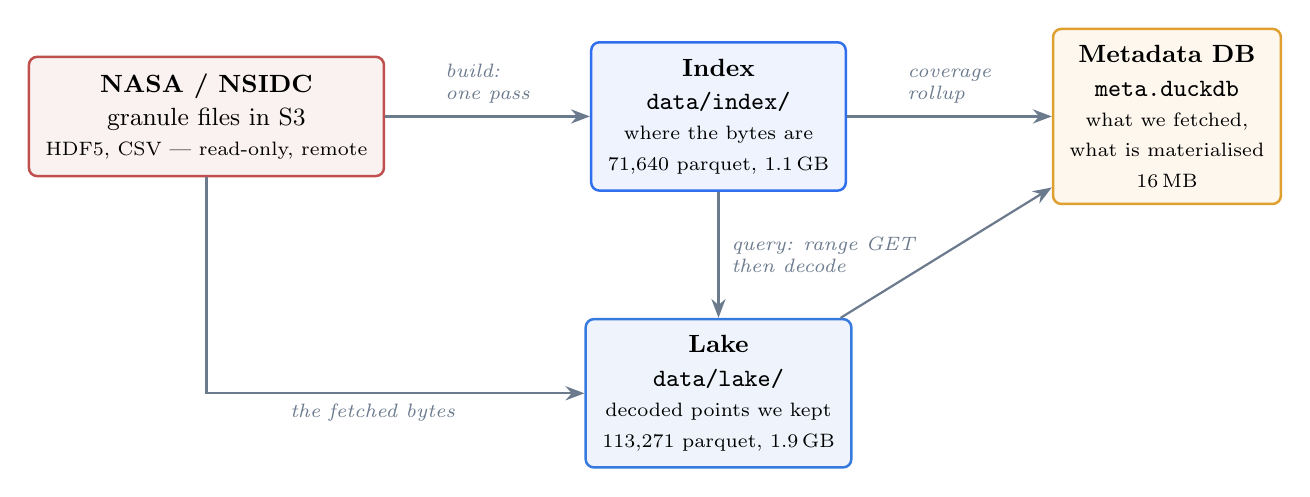
\begin{tikzpicture}[node distance=8mm]
  \node[store=nasared] (nasa) {\textbf{NASA / NSIDC}\\[1pt] granule files in S3\\ \scriptsize HDF5, CSV --- read-only, remote};
  \node[store=idxblue, right=26mm of nasa] (idx) {\textbf{Index}\\[1pt] \code{data/index/}\\ \scriptsize where the bytes are\\ \scriptsize 71{,}640 parquet, 1.1\,GB};
  \node[store=lakeblue, below=16mm of idx] (lake) {\textbf{Lake}\\[1pt] \code{data/lake/}\\ \scriptsize decoded points we kept\\ \scriptsize 113{,}271 parquet, 1.9\,GB};
  \node[store=metagold, right=26mm of idx] (meta) {\textbf{Metadata DB}\\[1pt] \code{meta.duckdb}\\ \scriptsize what we fetched,\\ \scriptsize what is materialised\\ \scriptsize 16\,MB};

  \draw[flow] (nasa) -- node[above, note, yshift=1pt] {build:\\one pass} (idx);
  \draw[flow] (idx) -- node[right, note, xshift=1pt] {query: range GET\\then decode} (lake);
  \draw[flow] (idx) -- node[above, note, yshift=1pt] {coverage\\rollup} (meta);
  \draw[flow] (lake) -- (meta);
  \draw[flow] (nasa.south) |- node[below, note, pos=0.72] {the fetched bytes} (lake.west);
\end{tikzpicture}
\end{center}

\begin{description}\setlength{\itemsep}{2pt}
\item[The index] is an \emph{address book}: never science values, only the coordinates of bytes. Built once
  per granule, then immutable. Unit: \(\bigl(\text{granule},\ \text{beam},\ \text{chunk},\ \text{cell}\bigr)\).
\item[The lake] is a \emph{cache of decoded points}. Losing it costs time, never truth --- anything missing is
  re-fetched. Unit: one Parquet file per \(\bigl(\text{granule},\text{beam},\text{chunk}\bigr)\) \emph{inside}
  one cell directory.
\item[The metadata DB] records \emph{what has been fetched} (so a chunk is never fetched twice) and
  \emph{what is materialised} (so sizing the lake need not walk it). Two different questions --- \S\ref{sec:meta}.
\end{description}

\section{The H3 grid}
\label{sec:h3key}

Every store is keyed on an H3 cell index: a 64-bit integer naming one hexagon on a global grid.

\begin{center}
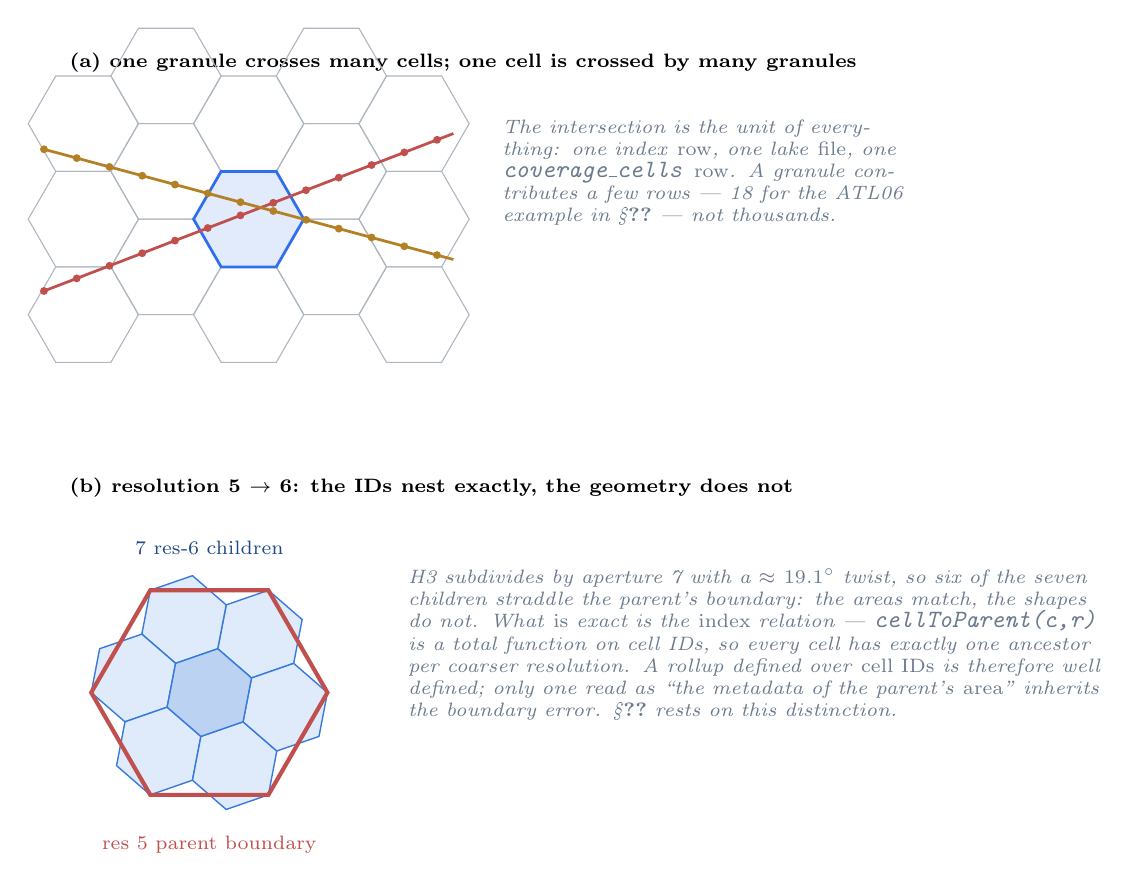
\begin{tikzpicture}[x=1mm, y=1mm, font=\footnotesize]

  %% ---------------- panel (a): tracks across cells ------------------------------------------
  \begin{scope}[shift={(0,0)}]
    \node[anchor=west, font=\scriptsize\bfseries] at (-3,32)
      {(a) one granule crosses many cells; one cell is crossed by many granules};
    \foreach \i in {0,2,4} { \foreach \j in {0,1,2} {
      \draw[draw=soft!55, line width=0.4pt] \hexp{10.5*\i}{12.124*\j}{7}{0}; } }
    \foreach \i in {1,3} { \foreach \j in {0,1,2} {
      \draw[draw=soft!55, line width=0.4pt] \hexp{10.5*\i}{12.124*\j+6.062}{7}{0}; } }
    \fill[idxblue!14] \hexp{21}{12.124}{7}{0};
    \draw[draw=idxblue, line width=1.0pt] \hexp{21}{12.124}{7}{0};

    \draw[draw=nasared, line width=1.0pt] (-5,3) -- (47,23);
    \foreach \s in {0,0.08,...,1.001} \fill[nasared] ({-5+52*\s},{3+20*\s}) circle (0.5);
    \draw[draw=metagold!80!black, line width=1.0pt] (-5,21) -- (47,7);
    \foreach \s in {0,0.08,...,1.001} \fill[metagold!80!black] ({-5+52*\s},{21-14*\s}) circle (0.5);

    \node[note, anchor=north west, text width=52mm] at (52,26)
      {The intersection is the unit of everything: one index \emph{row}, one lake \emph{file}, one
       \code{coverage\_cells} \emph{row}. A granule contributes a few rows --- 18 for the ATL06 example in
       \S\ref{sec:chunkmap} --- not thousands.};
  \end{scope}

  %% ---------------- panel (b): the ID hierarchy ---------------------------------------------
  \begin{scope}[shift={(16,-48)}]
    \node[anchor=west, font=\scriptsize\bfseries] at (-19,26)
      {(b) resolution 5 $\rightarrow$ 6: the IDs nest exactly, the geometry does not};
    % NB: \hexp uses \k internally, so this loop must not.
    \foreach \m in {0,...,5} {
      \fill[lakeblue!16] \hexp{9.821*cos(49.106+60*\m)}{9.821*sin(49.106+60*\m)}{5.669}{19.106};
      \draw[draw=lakeblue, line width=0.5pt]
        \hexp{9.821*cos(49.106+60*\m)}{9.821*sin(49.106+60*\m)}{5.669}{19.106}; }
    \fill[lakeblue!34] \hexp{0}{0}{5.669}{19.106};
    \draw[draw=lakeblue, line width=0.5pt] \hexp{0}{0}{5.669}{19.106};
    \draw[draw=nasared, line width=1.5pt] \hexp{0}{0}{15}{0};
    \node[font=\scriptsize, text=nasared, anchor=north] at (0,-17) {res 5 parent boundary};
    \node[font=\scriptsize, text=lakeblue!60!black, anchor=north] at (0,20.5) {7 res-6 children};

    \node[note, anchor=north west, text width=88mm] at (24,17)
      {H3 subdivides by aperture 7 with a $\approx19.1^{\circ}$ twist, so six of the seven children straddle
       the parent's boundary: the areas match, the shapes do not. What \emph{is} exact is the \emph{index}
       relation --- \code{cellToParent(c,r)} is a total function on cell IDs, so every cell has exactly one
       ancestor per coarser resolution. A rollup defined over \emph{cell IDs} is therefore well defined; only
       one read as ``the metadata of the parent's \emph{area}'' inherits the boundary error.
       \S\ref{sec:h3} rests on this distinction.};
  \end{scope}
\end{tikzpicture}
\end{center}

\begin{center}\small
\begin{tabular}{@{}llrrrr@{}}
\toprule
\textbf{Collection} & \textbf{Product} & \textbf{Res} & \textbf{Cells on the globe} & \textbf{Mean area} & \textbf{Mean edge} \\
\midrule
\code{ATL06}   & ICESat-2 ATL06 land ice & 5 & 2{,}016{,}842  & 252.9\,km$^2$ & 9.85\,km \\
\code{GLAS}    & ICESat/GLAS GLAH06      & 5 & 2{,}016{,}842  & 252.9\,km$^2$ & 9.85\,km \\
\code{ICESSN}  & IceBridge ATM ILATM2    & 5 & 2{,}016{,}842  & 252.9\,km$^2$ & 9.85\,km \\
\code{ATL03}   & ICESat-2 ATL03 photons  & 6 & 14{,}117{,}882 & 36.1\,km$^2$  & 3.73\,km \\
\bottomrule
\end{tabular}
\end{center}

\noindent
The dense photon product is indexed one resolution finer because a res-5 cell holds far too many photons to
be a useful fetch unit. Within a collection the index and lake resolutions are deliberately \emph{equal}: a
lake file is written at the same resolution its index row named, so a later query for a different sub-box
inside that cell re-filters correctly instead of returning a partial cell.

\section{The index}

\subsection{Directory layout}

\begin{center}
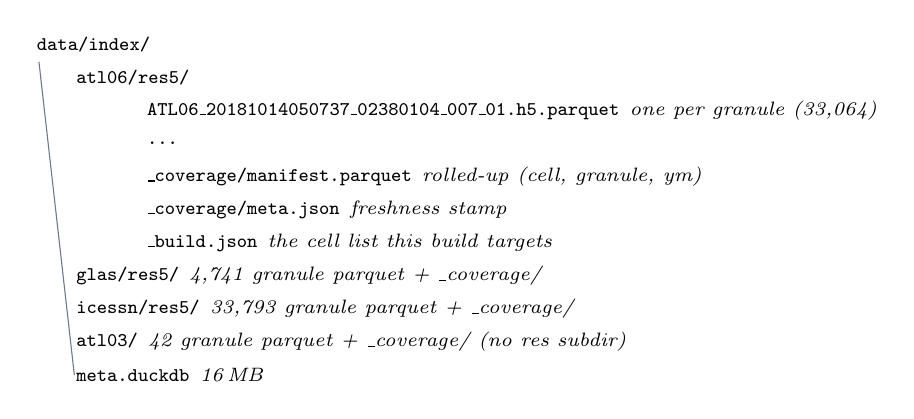
\begin{tikzpicture}[node distance=1mm, every node/.style={font=\ttfamily\scriptsize, anchor=west}]
  \node (a) at (0,0)        {data/index/};
  \node (b) at (0.5,-0.42)  {atl06/res5/};
  \node (b1) at (1.4,-0.84) {ATL06\_20181014050737\_02380104\_007\_01.h5.parquet \normalfont\itshape one per granule (33{,}064)};
  \node (b2) at (1.4,-1.26) {\dots};
  \node (b3) at (1.4,-1.68) {\_coverage/manifest.parquet \normalfont\itshape rolled-up (cell, granule, ym)};
  \node (b4) at (1.4,-2.10) {\_coverage/meta.json \normalfont\itshape freshness stamp};
  \node (b5) at (1.4,-2.52) {\_build.json \normalfont\itshape the cell list this build targets};
  \node (c) at (0.5,-2.94)  {glas/res5/ \normalfont\itshape 4{,}741 granule parquet + \_coverage/};
  \node (d) at (0.5,-3.36)  {icessn/res5/ \normalfont\itshape 33{,}793 granule parquet + \_coverage/};
  \node (e) at (0.5,-3.78)  {atl03/ \normalfont\itshape 42 granule parquet + \_coverage/ (no res subdir)};
  \node (f) at (0.5,-4.20)  {meta.duckdb \normalfont\itshape 16\,MB};
  \draw[draw=soft, line width=0.4pt] ($(a.south west)+(0.15,0)$) -- ($(f.west)+(0.1,0)$);
\end{tikzpicture}
\end{center}

\noindent
Each collection directory is \emph{flat}: one Parquet file per granule, named \code{<granule>.parquet} with
the granule's own \code{.h5}\,/\,\code{.csv} suffix retained. Two consequences, both of which have bitten:

\begin{enumerate}\setlength{\itemsep}{2pt}
\item Files land \textbf{tmp-then-rename}, so a reader never sees a torn Parquet and the \emph{directory}
  mtime moves whenever a granule arrives. That single \code{stat()} is the freshness gate used everywhere
  downstream (\S\ref{sec:freshness}).
\item Anything that answers a question by opening every file does work proportional to the \emph{store}, not
  the \emph{request} --- 43.5\,s at 33{,}064 files. The \code{\_coverage/} rollup exists to stop that, and
  sits in a \emph{subdirectory} so a \code{*.parquet} glob cannot pick up a schema-mismatched file and so
  writing it does not invalidate its own freshness stamp.
\end{enumerate}

\subsection{The chunk map: from an HDF5 file to index rows}
\label{sec:chunkmap}

An HDF5 dataset is stored as fixed-length chunks along its first axis, each compressed independently and
placed wherever the writer had room. The \emph{chunk map} is the dataset's B-tree read out as a list: for
chunk $k$, its byte offset, its compressed size, and its filter mask. \code{\_chunk\_manifest} walks that
B-tree once per dataset --- the only time a granule's B-trees are ever read --- and sorts the result into
\emph{logical} order, so entry $k$ is the $k$-th chunk along the axis regardless of where it sits in the file.

\begin{center}
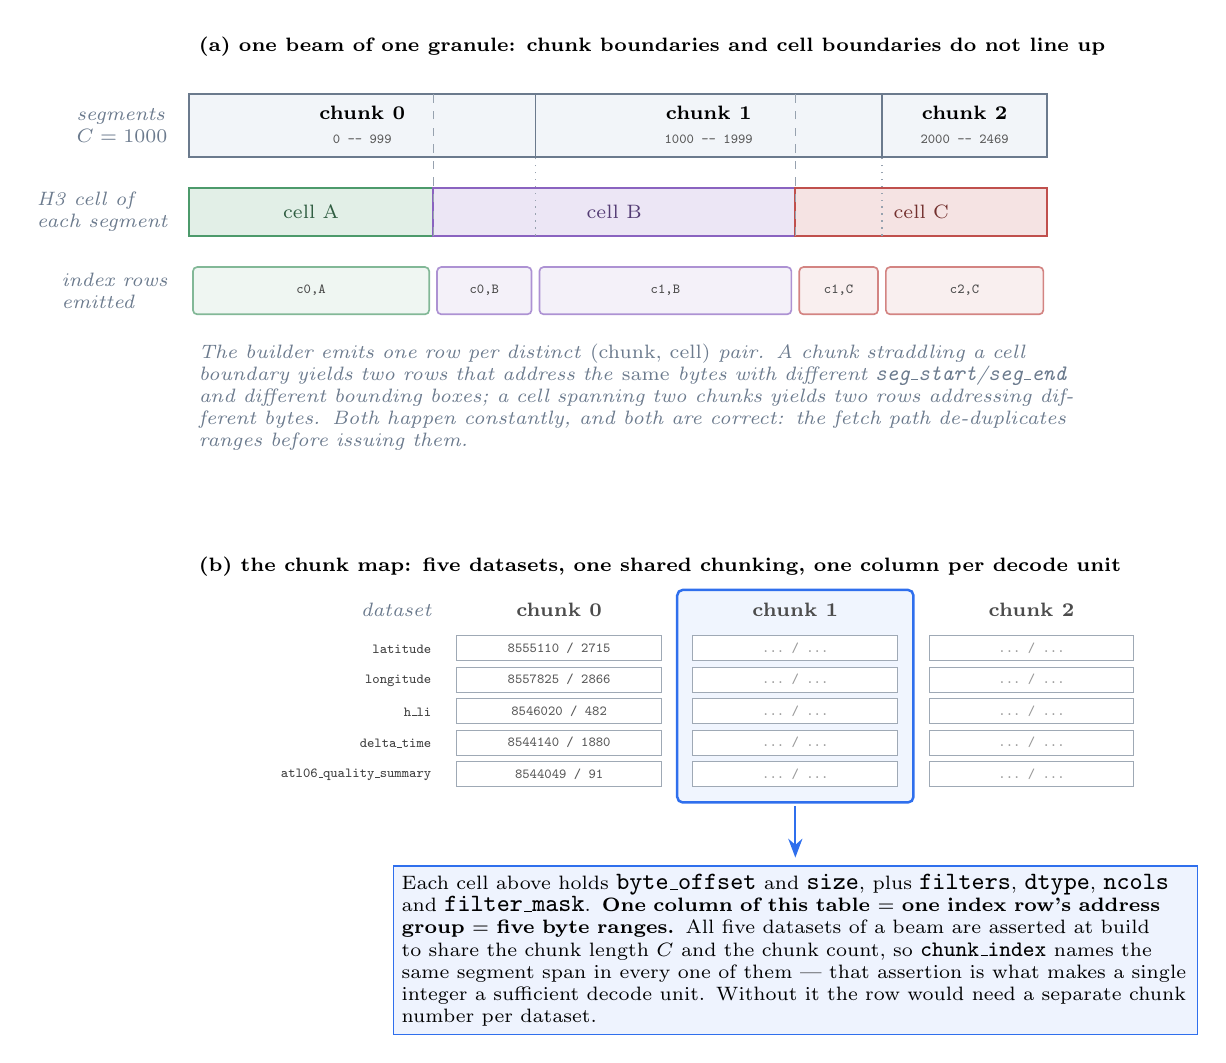
\begin{tikzpicture}[x=1mm, y=1mm, font=\footnotesize]

  %% ---- panel (a): logical axis, cells, and the rows that fall out --------------------------
  \node[anchor=west, font=\scriptsize\bfseries] at (0,40)
    {(a) one beam of one granule: chunk boundaries and cell boundaries do not line up};

  % the segment axis, cut into chunks
  \foreach \x/\w/\k/\lbl in {0/44/0/{0 -- 999}, 44/44/1/{1000 -- 1999}, 88/21/2/{2000 -- 2469}} {
    \draw[draw=soft, fill=panel, line width=0.7pt] (\x,26) rectangle (\x+\w,34);
    \node[font=\scriptsize\bfseries] at (\x+\w/2,31.6) {chunk \k};
    \node[font=\ttfamily\tiny, text=black!65] at (\x+\w/2,28.2) {\lbl};
  }
  \node[note, anchor=east] at (-1.5,30) {segments\\$C=1000$};

  % the cell runs underneath
  \foreach \x/\w/\c/\lbl in {0/31/cellA/{cell A}, 31/46/cellB/{cell B}, 77/32/nasared/{cell C}} {
    \draw[draw=\c, fill=\c!16, line width=0.7pt] (\x,16) rectangle (\x+\w,22);
    \node[font=\scriptsize, text=\c!60!black] at (\x+\w/2,19) {\lbl};
  }
  \node[note, anchor=east] at (-1.5,19) {H3 cell of\\each segment};
  \foreach \x in {31,77} { \draw[draw=soft!70, dashed, line width=0.4pt] (\x,16) -- (\x,34); }
  \foreach \x in {44,88} { \draw[draw=soft!70, dotted, line width=0.5pt] (\x,16) -- (\x,26); }

  % the resulting rows
  \foreach \x/\w/\c/\lbl in {0/31/cellA/{c0,A}, 31/13/cellB/{c0,B}, 44/33/cellB/{c1,B},
                             77/11/nasared/{c1,C}, 88/21/nasared/{c2,C}} {
    \draw[draw=\c!70, fill=\c!9, line width=0.6pt, rounded corners=1.5pt] (\x+0.5,6) rectangle (\x+\w-0.5,12);
    \node[font=\ttfamily\tiny, text=black!70] at (\x+\w/2,9) {\lbl};
  }
  \node[note, anchor=east] at (-1.5,9) {index rows\\emitted};
  \node[note, anchor=north west, text width=112mm] at (0,3.5)
    {The builder emits one row per distinct \emph{(chunk, cell)} pair. A chunk straddling a cell boundary
     yields two rows that address the \emph{same} bytes with different \col{seg\_start}/\col{seg\_end} and
     different bounding boxes; a cell spanning two chunks yields two rows addressing different bytes. Both
     happen constantly, and both are correct: the fetch path de-duplicates ranges before issuing them.};

  %% ---- panel (b): the chunk map itself -----------------------------------------------------
  \begin{scope}[shift={(0,-58)}]
    \node[anchor=west, font=\scriptsize\bfseries] at (0,32)
      {(b) the chunk map: five datasets, one shared chunking, one column per decode unit};

    \draw[draw=idxblue, fill=idxblue!7, line width=0.9pt, rounded corners=2pt] (62,2) rectangle (92,29);
    \foreach \n/\x in {0/34, 1/64, 2/94} {
      \node[font=\scriptsize\bfseries, text=black!70] at (\x+13,26.5) {chunk \n}; }

    \foreach \d/\y/\o/\s in {latitude/20/8555110/2715, longitude/16/8557825/2866, h\_li/12/8546020/482,
                             delta\_time/8/8544140/1880, atl06\_quality\_summary/4/8544049/91} {
      \node[anchor=east, font=\ttfamily\tiny, text=black!75] at (32,\y+1.5) {\d};
      \foreach \x in {34,64,94} {
        \draw[draw=soft!65, fill=white, line width=0.35pt] (\x,\y) rectangle (\x+26,\y+3.2); }
      \node[font=\ttfamily\tiny, text=black!65] at (47,\y+1.6) {\o\ /\ \s};
      \node[font=\ttfamily\tiny, text=black!40] at (77,\y+1.6) {\dots\ /\ \dots};
      \node[font=\ttfamily\tiny, text=black!40] at (107,\y+1.6) {\dots\ /\ \dots};
    }
    \node[anchor=east, font=\scriptsize\itshape, text=soft] at (32,26.5) {dataset};

    \draw[flow, draw=idxblue] (77,1.5) -- (77,-5);
    \node[bit, anchor=north, fill=idxblue!8, draw=idxblue, align=left, text width=100mm] at (77,-6)
      {Each cell above holds \code{byte\_offset} and \code{size}, plus \code{filters}, \code{dtype},
       \code{ncols} and \code{filter\_mask}. \textbf{One column of this table $=$ one index row's
       \textsc{address} group $=$ five byte ranges.} All five datasets of a beam are asserted at build to
       share the chunk length $C$ and the chunk count, so \col{chunk\_index} names the same segment span in
       every one of them --- that assertion is what makes a single integer a sufficient decode unit. Without
       it the row would need a separate chunk number per dataset.};
  \end{scope}
\end{tikzpicture}
\end{center}

\noindent
Chunk numbering is logical, byte placement is not: the five ranges of one chunk usually sit close together
(they were written together) but the chunks of one dataset are not necessarily in file order, and ATL03's
ranges can be gigabytes apart. That is why the fetch path sorts and coalesces ranges with a gap threshold
rather than assuming adjacency --- \S\ref{sec:bytes}.

\subsection{What is in one index Parquet file}

\begin{center}
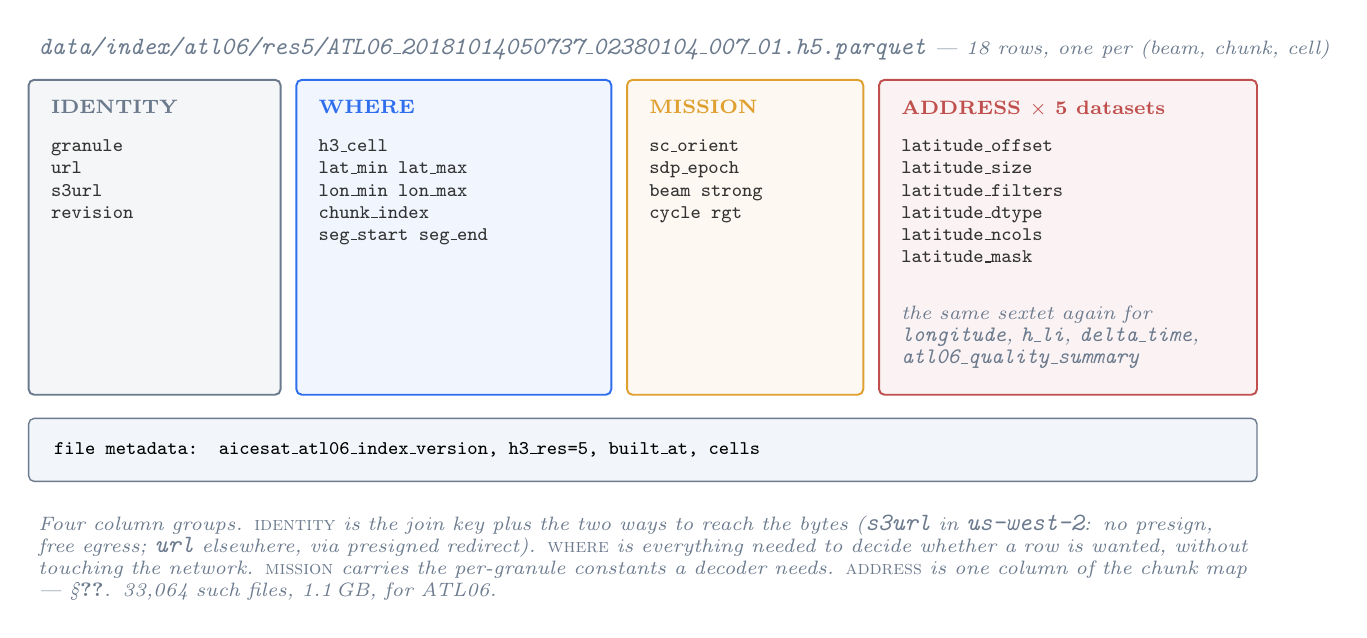
\begin{tikzpicture}[x=1mm, y=1mm, font=\scriptsize]
  \node[note, anchor=west] at (0,4)
    {\code{data/index/atl06/res5/ATL06\_20181014050737\_02380104\_007\_01.h5.parquet} --- 18 rows, one per
     (beam, chunk, cell)};

  \foreach \x/\w/\c/\t/\body in {%
     0/32/soft/IDENTITY/{granule\\url\\s3url\\revision},
    34/40/idxblue/WHERE/{h3\_cell\\lat\_min lat\_max\\lon\_min lon\_max\\chunk\_index\\seg\_start seg\_end},
    76/30/metagold/MISSION/{sc\_orient\\sdp\_epoch\\beam strong\\cycle rgt},
   108/48/nasared/{ADDRESS $\times$ 5 datasets}/{latitude\_offset\\latitude\_size\\latitude\_filters\\latitude\_dtype\\latitude\_ncols\\latitude\_mask}%
  } {
    \draw[draw=\c, fill=\c!7, line width=0.7pt, rounded corners=2pt] (\x,-40) rectangle (\x+\w,0);
    \node[hdr=\c, anchor=north west] at (\x+1.6,-1.4) {\t};
    \node[anchor=north west, font=\ttfamily\scriptsize, align=left, text=black!80] at (\x+1.6,-6.4) {\body};
  }
  \node[note, anchor=north west, text width=44mm] at (109.6,-27.5)
    {the same sextet again for\\ \col{longitude}, \col{h\_li}, \col{delta\_time},\\ \col{atl06\_quality\_summary}};

  \draw[draw=soft, fill=panel, line width=0.5pt, rounded corners=2pt] (0,-51) rectangle (156,-43);
  \node[anchor=west, font=\ttfamily\scriptsize] at (2,-47)
    {file metadata: aicesat\_atl06\_index\_version, h3\_res=5, built\_at, cells};
  \node[note, anchor=north west, text width=156mm] at (0,-54)
    {Four column groups. \textsc{identity} is the join key plus the two ways to reach the bytes
     (\code{s3url} in \code{us-west-2}: no presign, free egress; \code{url} elsewhere, via presigned
     redirect). \textsc{where} is everything needed to decide whether a row is wanted, without touching the
     network. \textsc{mission} carries the per-granule constants a decoder needs. \textsc{address} is one
     column of the chunk map --- \S\ref{sec:chunkmap}. 33{,}064 such files, 1.1\,GB, for ATL06.};
\end{tikzpicture}
\end{center}

\vspace{2mm}
\noindent
Only the \textsc{address} group differs between collections:

\begin{center}\small
\begin{tabular}{@{}p{20mm}p{32mm}p{72mm}@{}}
\toprule
\textbf{Collection} & \textbf{Row grain} & \textbf{Address columns} \\
\midrule
\code{ATL06}, \code{ATL03} & (granule, beam, chunk, cell) &
  per dataset: \col{\_offset} \col{\_size} \col{\_filters} \col{\_dtype} \col{\_ncols} \col{\_mask}.
  HDF5 chunk ranges. \col{\_ncols} matters: ATL03's \col{signal\_conf\_ph} is $n\times5$. \\
\addlinespace[2pt]
\code{GLAS} & (granule, beam=\code{na}, chunk, cell) &
  the same, with \col{\_fill} instead of \col{\_ncols}: GLAH06 encodes no-data as
  $1.798\times10^{308}$, not NaN. \\
\addlinespace[2pt]
\code{ICESSN} & (granule, cell) &
  \col{byte\_start} \col{byte\_end} \col{n\_lines}. Plain CSV --- a line range, no chunk map at all. \\
\bottomrule
\end{tabular}
\end{center}

\noindent
GLAS and ICESSN replace the \textsc{mission} group with \col{gdate} (\code{YYYYMMDD}), having no
repeat-cycle number; ATL03 replaces \col{seg\_start}/\col{seg\_end} with \col{ph\_start}/\col{ph\_end}.
Row counts per granule stay small --- 18 (ATL06), 7 (ATL03), 25 (GLAS), 2 (ICESSN) --- so the whole index is
1.1\,GB across 71{,}640 granules.

\subsection{Byte-range addressing}
\label{sec:bytes}

\begin{center}
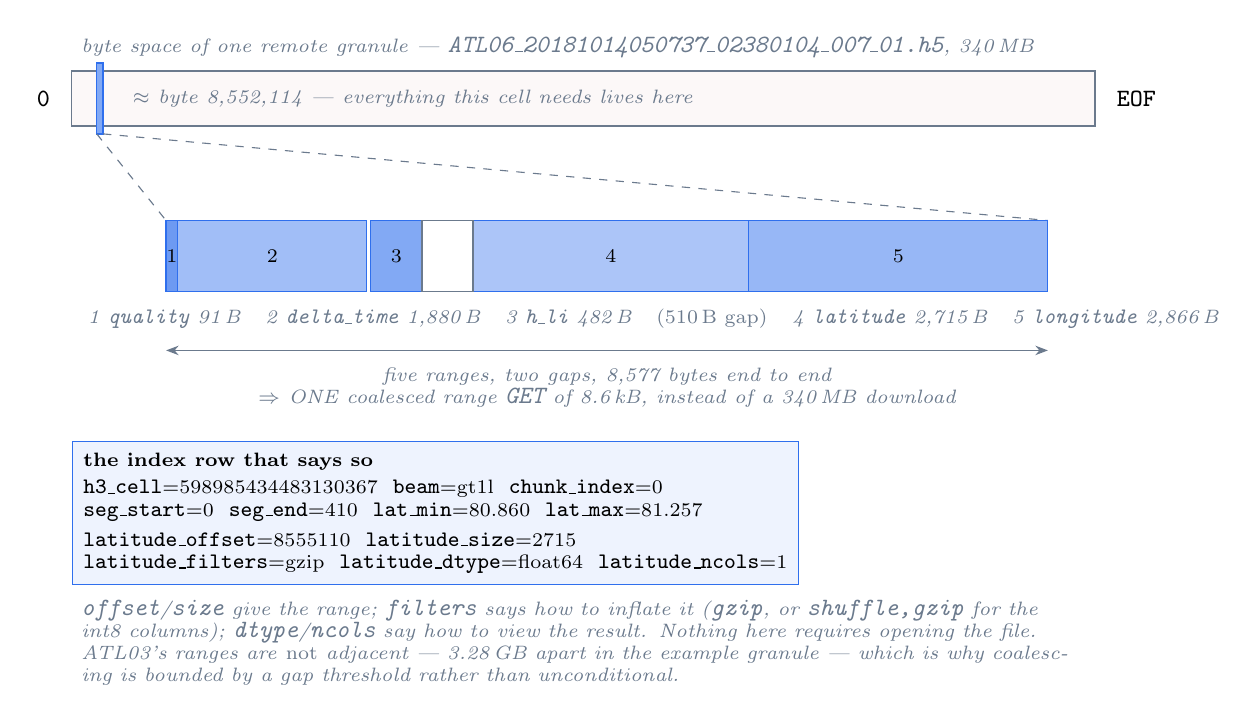
\begin{tikzpicture}[x=1mm, y=1mm, font=\footnotesize]
  \node[note, anchor=west] at (0,50)
    {byte space of one remote granule --- \code{ATL06\_20181014050737\_02380104\_007\_01.h5}, 340\,MB};
  \draw[draw=soft, fill=nasared!4, line width=0.6pt] (0,40) rectangle (130,47);
  \node[font=\scriptsize, anchor=east] at (-1.5,43.5) {\code{0}};
  \node[font=\scriptsize, anchor=west] at (131.5,43.5) {\code{EOF}};
  \draw[fill=idxblue!60, draw=idxblue, line width=0.5pt] (3.2,39) rectangle (4.0,48);
  \node[note, anchor=west] at (6.5,43.5) {$\approx$ byte 8{,}552{,}114 --- everything this cell needs lives here};

  \draw[draw=soft, dashed, line width=0.4pt] (3.2,39) -- (12,28);
  \draw[draw=soft, dashed, line width=0.4pt] (4.0,39) -- (124,28);
  \foreach \a/\b/\n/\c in {12/13.5/1/70, 13.5/37.5/2/45, 38.0/44.5/3/60, 51.0/86.0/4/40, 86.0/124/5/50} {
    \draw[fill=idxblue!\c, draw=idxblue, line width=0.4pt] (\a,19) rectangle (\b,28);
    \node[font=\scriptsize] at ({(\a+\b)/2},23.5) {\n};
  }
  \draw[draw=soft, line width=0.5pt] (44.5,19) rectangle (51.0,28);
  \node[note, anchor=west] at (0,15.5)
    {\;1 \col{quality} 91\,B \ \ 2 \col{delta\_time} 1{,}880\,B \ \ 3 \col{h\_li} 482\,B \ \
      \emph{(510\,B gap)} \ \ 4 \col{latitude} 2{,}715\,B \ \ 5 \col{longitude} 2{,}866\,B};
  \draw[{Stealth[length=1.6mm]}-{Stealth[length=1.6mm]}, draw=soft, line width=0.5pt] (12,11.5) -- (124,11.5);
  \node[note, anchor=north, align=center] at (68,10.5) {five ranges, two gaps, 8{,}577 bytes end to end\\
    $\Rightarrow$ ONE coalesced range \code{GET} of 8.6\,kB, instead of a 340\,MB download};

  \node[bit, anchor=north west, fill=idxblue!8, draw=idxblue, align=left, inner sep=4pt] (row) at (0,0)
    {\textbf{the index row that says so}\\[2pt]
     \col{h3\_cell}=598985434483130367\ \ \col{beam}=gt1l\ \ \col{chunk\_index}=0\\
     \col{seg\_start}=0\ \ \col{seg\_end}=410\ \ \col{lat\_min}=80.860\ \ \col{lat\_max}=81.257\\[3pt]
     \col{latitude\_offset}=8555110\ \ \col{latitude\_size}=2715\\
     \col{latitude\_filters}=gzip\ \ \col{latitude\_dtype}=float64\ \ \col{latitude\_ncols}=1};
  \node[note, anchor=north west, text width=128mm] at (0,-19)
    {\code{offset}/\code{size} give the range; \code{filters} says how to inflate it (\code{gzip}, or
     \code{shuffle,gzip} for the int8 columns); \code{dtype}/\code{ncols} say how to view the result. Nothing
     here requires opening the file. ATL03's ranges are \emph{not} adjacent --- 3.28\,GB apart in the example
     granule --- which is why coalescing is bounded by a gap threshold rather than unconditional.};
\end{tikzpicture}
\end{center}

\subsection{The coverage manifest}
\label{sec:freshness}

Answering ``which cells does this collection cover, over what period?'' from the per-granule files means
opening all of them. \code{<index dir>/\_coverage/manifest.parquet} is the rollup that avoids it: the
\code{DISTINCT} triples \col{h3\_cell} (uint64), \col{granule} (string), \col{ym} (\code{YYYY-MM}, from
\col{gdate} for GLAS/ICESSN, parsed out of the granule \emph{name} for ATL0x). For ATL06 that is
2{,}261{,}439 rows in 27\,MB, against 33{,}064 files and 1.1\,GB.

\begin{center}
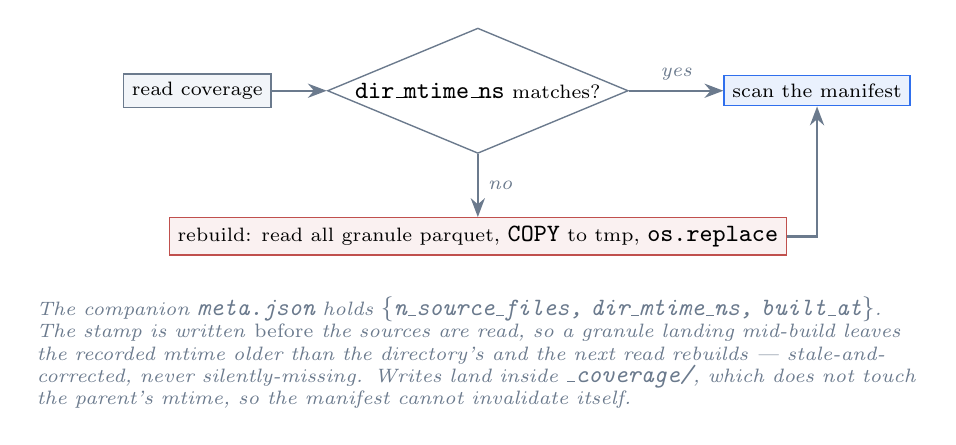
\begin{tikzpicture}[node distance=7mm]
  \node[bit, fill=panel] (q) {read coverage};
  \node[bit, right=of q, diamond, aspect=2.4, inner sep=1pt] (chk) {\code{dir\_mtime\_ns} matches?};
  \node[bit, right=12mm of chk, fill=idxblue!10, draw=idxblue] (use) {scan the manifest};
  \node[bit, below=8mm of chk, fill=nasared!8, draw=nasared] (build) {rebuild: read all granule parquet, \code{COPY} to tmp, \code{os.replace}};
  \draw[flow] (q) -- (chk);
  \draw[flow] (chk) -- node[above, note] {yes} (use);
  \draw[flow] (chk) -- node[right, note] {no} (build);
  \draw[flow] (build) -| (use);
  \node[note, below=4mm of build.south, text width=112mm, anchor=north]
    {The companion \code{meta.json} holds \code{\{n\_source\_files, dir\_mtime\_ns, built\_at\}}. The stamp is
     written \emph{before} the sources are read, so a granule landing mid-build leaves the recorded mtime
     older than the directory's and the next read rebuilds --- stale-and-corrected, never silently-missing.
     Writes land inside \code{\_coverage/}, which does not touch the parent's mtime, so the manifest cannot
     invalidate itself.};
\end{tikzpicture}
\end{center}

\noindent
\textbf{Known lag.} The rebuild being lazy, the manifest trails the directory by a few granules between
builds: 33{,}053 vs 33{,}064 (ATL06), 4{,}649 vs 4{,}741 (GLAS), 33{,}578 vs 33{,}793 (ICESSN). Those
granules fall in already-covered cells, so the \emph{cell set} is unaffected (14{,}482 / 23{,}142 / 7{,}782,
identical either way). Counts that must be exact --- notably the ``index build $N\%$ done'' readout --- come
from a directory listing instead.

\section{The lake}

\subsection{Layout and naming}

\begin{center}
\begin{Verbatim}[fontsize=\scriptsize, frame=single, framesep=3mm, rulecolor=\color{soft}]
data/lake/mission=ATL06/h3_cell=599100951923523583/
    ATL06_20181119053215_07880105_007_01__gt1l__c5.parquet   <- granule __ beam __ chunk
    ATL06_20181119053215_07880105_007_01__gt1r__c5.parquet
    ...                                                       (656 files in this cell)
data/lake/mission=ICESAT2/h3_cell=604538106045005823/
    ATL03_20210830193051_10411206_007_01.h5__gt2r.parquet     <- granule __ beam  (NO chunk)
\end{Verbatim}
\end{center}

\noindent
Hive-style partitioning, so DuckDB prunes on \code{mission=} and \code{h3\_cell=} without reading anything.
The file name is the write's identity, which makes re-materialisation idempotent by construction.

\paragraph{The photon path names files differently, and it matters.}
\code{write\_point\_chunk} (ATL06 / GLAS / ICESSN) emits one file per
\((\text{granule},\text{beam},\text{chunk})\), so one coverage row is exactly one file.
\code{write\_photons} (ATL03, under \code{mission=ICESAT2}) omits the chunk, so \emph{many} coverage rows map
to \emph{one} file: 390 rows against 363 files. Any scheme deriving per-file quantities by summing per-row
quantities is wrong on this path.

\subsection{What is in one lake Parquet file}

\begin{center}
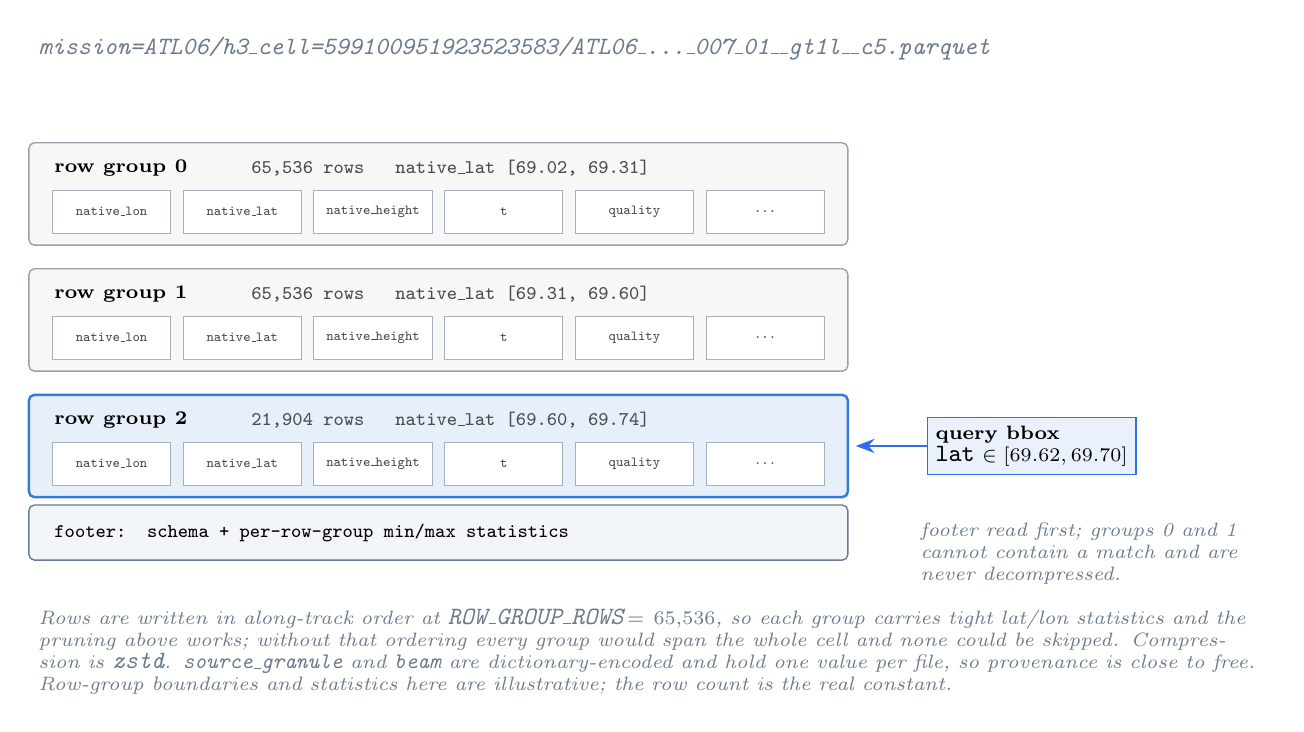
\begin{tikzpicture}[x=1mm, y=1mm, font=\scriptsize]
  \node[note, anchor=west] at (0,4) {\code{mission=ATL06/h3\_cell=599100951923523583/ATL06\_\dots\_007\_01\_\_gt1l\_\_c5.parquet}};

  \foreach \j/\y/\rows/\latlo/\lathi/\dc/\fc/\lw in {%
      0/-8/{65{,}536}/69.02/69.31/{soft!70}/{black!3}/0.5,
      1/-24/{65{,}536}/69.31/69.60/{soft!70}/{black!3}/0.5,
      2/-40/{21{,}904}/69.60/69.74/{lakeblue}/{lakeblue!12}/0.9} {
    \draw[draw=\dc, fill=\fc, line width=\lw pt, rounded corners=2pt] (0,\y-13) rectangle (104,\y);
    \node[anchor=north west, font=\scriptsize\bfseries] at (2,\y-1) {row group \j};
    \node[anchor=north west, font=\ttfamily\scriptsize, text=black!70] at (27,\y-1)
      {\rows\ rows \ \ native\_lat [\latlo, \lathi]};
    \foreach \k/\cn in {0/native\_lon, 1/native\_lat, 2/native\_height, 3/t, 4/quality, 5/\dots} {
      \draw[draw=soft!60, fill=white, line width=0.35pt] ({3+16.6*\k},\y-11.5) rectangle ({3+16.6*\k+15},\y-6);
      \node[font=\ttfamily\tiny, text=black!70] at ({3+16.6*\k+7.5},\y-8.75) {\cn}; }
  }
  \draw[draw=soft, fill=panel, line width=0.5pt, rounded corners=2pt] (0,-61) rectangle (104,-54);
  \node[anchor=west, font=\ttfamily\scriptsize] at (2,-57.5) {footer: schema + per-row-group min/max statistics};

  \node[bit, anchor=west, fill=idxblue!10, draw=idxblue, align=left] (pred) at (114,-46.5)
    {\textbf{query bbox}\\\code{lat} $\in [69.62, 69.70]$};
  \draw[flow, draw=idxblue] (pred.west) -- (105,-46.5);
  \node[note, anchor=north west, text width=42mm] at (112,-55)
    {footer read first; groups 0 and 1 cannot contain a match and are never decompressed.};

  \node[note, anchor=north west, text width=156mm] at (0,-66)
    {Rows are written in along-track order at \code{ROW\_GROUP\_ROWS}\,$=65{,}536$, so each group carries
     tight lat/lon statistics and the pruning above works; without that ordering every group would span the
     whole cell and none could be skipped. Compression is \code{zstd}. \col{source\_granule} and \col{beam}
     are dictionary-encoded and hold one value per file, so provenance is close to free. Row-group boundaries
     and statistics here are illustrative; the row count is the real constant.};
\end{tikzpicture}
\end{center}

\vspace{2mm}
\begin{center}\small
\begin{tabular}{@{}llp{74mm}@{}}
\toprule
\textbf{Column} & \textbf{Type} & \textbf{Meaning} \\
\midrule
\col{native\_lon}, \col{native\_lat} & double & position as published, never rewritten \\
\col{native\_height}                 & double & elevation in the source's own datum \\
\col{t}                              & timestamp[ms] & observation time \\
\col{source\_granule}, \col{beam}    & dictionary & provenance, one value per file \\
\col{source\_chunk\_index}           & int32  & which fetch unit produced this row \\
\midrule
\multicolumn{3}{@{}l}{\emph{ATL06 adds}} \\
\col{quality}                        & int8   & \code{atl06\_quality\_summary} \\
\multicolumn{3}{@{}l}{\emph{ICESSN adds}} \\
\col{sn\_slope}, \col{we\_slope}     & double & along/across-track surface slope \\
\multicolumn{3}{@{}l}{\emph{ICESAT2 (ATL03 photons) adds}} \\
\col{row\_id}                        & uint64 & \code{crc32(granule/beam)} $\ll32$ $\mid$ photon index --- a
                                                deterministic surrogate key \\
\col{height\_ref}, \col{native\_frame} & dictionary & e.g.\ \code{WGS84 ellipsoid}, \code{ITRF2014} \\
\col{coreg\_lon}, \col{coreg\_lat}, \col{coreg\_epoch} & double & co-registered position at
                                                \code{COMMON\_EPOCH} $=2005.0$, materialised at ingest \\
\col{signal\_conf\_landice}          & int8   & photon confidence \\
\col{photon\_index}                  & int64  & index within the granule/beam \\
\bottomrule
\end{tabular}
\end{center}

\section{The metadata database}
\label{sec:meta}

\code{data/index/meta.duckdb} holds two tables answering two \emph{different} questions. Conflating them is
the single most productive source of bugs in this subsystem.

\begin{center}\small
\begin{tabular}{@{}llp{72mm}@{}}
\toprule
\multicolumn{3}{@{}l}{\code{coverage\_cells} --- \emph{what has been fetched}. 118{,}157 rows.} \\
\midrule
\col{mission} & VARCHAR & \code{ATL06} / \code{GLAS} / \code{ICESSN} / \code{ICESAT2} \\
\col{granule}, \col{beam} & VARCHAR & \col{beam}\,=\,\code{na} where the source has no beams \\
\col{chunk\_index} & INTEGER & \\
\col{h3\_cell} & UBIGINT & \\
\col{ingested\_at} & TIMESTAMP & \\
\multicolumn{3}{@{}l}{\footnotesize PK \((\text{mission},\text{granule},\text{beam},\text{chunk\_index},\text{h3\_cell})\)} \\
\addlinespace[4pt]
\multicolumn{3}{@{}l}{\code{lake\_cell\_stats} --- \emph{what is materialised}. One row per cell.} \\
\midrule
\col{mission}, \col{h3\_cell} & VARCHAR, UBIGINT & PK \\
\col{dir\_mtime\_ns} & HUGEINT & the cell directory's mtime this rollup was computed at \\
\col{rows\_known}    & BOOLEAN & false when computed by a cheap pass that skipped row counts \\
\col{files}, \col{n\_rows}, \col{n\_bytes} & INTEGER, BIGINT, BIGINT & \\
\col{granules}, \col{beams} & VARCHAR[] & \\
\bottomrule
\end{tabular}
\end{center}

\paragraph{Why \code{coverage\_cells} cannot size the lake.}
It deliberately records cells a chunk \emph{wanted} but wrote nothing to --- \code{index\_atl06} marks every
wanted cell of a fetched chunk ``so an all-fill cell is not re-fetched forever'', and the writer then drops
non-finite positions and, for ATL06, segments with \code{quality} $\neq 0$. Measured on the deployed lake:
\textbf{4{,}373 of 107{,}363 ATL06 rows (4.1\%) name a file that does not exist}, over 184 cells and 922
granules --- and every file on disk has a row (zero unmarked). Not drift, not eviction: a faithful record of
a different fact. Hence the separate rollup table.

\begin{center}
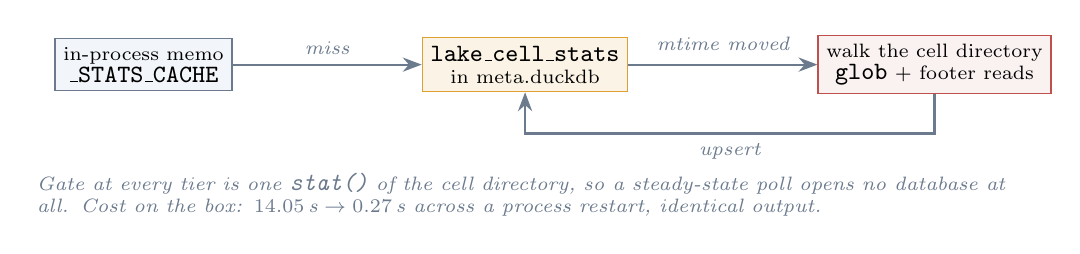
\begin{tikzpicture}[node distance=6mm]
  \node[bit, fill=panel] (a) {in-process memo\\\code{\_STATS\_CACHE}};
  \node[bit, right=24mm of a, fill=metagold!12, draw=metagold] (b) {\code{lake\_cell\_stats}\\in meta.duckdb};
  \node[bit, right=24mm of b, fill=nasared!8, draw=nasared] (c) {walk the cell directory\\\code{glob} + footer reads};
  \draw[flow] (a) -- node[above, note] {miss} (b);
  \draw[flow] (b) -- node[above, note, yshift=0.5mm] {mtime moved} (c);
  \draw[flow] (c.south) -- ++(0,-5mm) -| node[below, note, pos=0.25] {upsert} (b.south);
  \node[note, below=9mm of b.south, text width=124mm, anchor=north]
    {Gate at every tier is one \code{stat()} of the cell directory, so a steady-state poll opens no database
     at all. Cost on the box: \(14.05\,\text{s} \rightarrow 0.27\,\text{s}\) across a process restart,
     identical output.};
\end{tikzpicture}
\end{center}

\section{Read paths and what they cost}

Measured on the deployed \code{t3.large} in \code{us-west-2}, against 102{,}990 lake files and 71{,}640 index
parquet.

\begin{center}\small
\begin{tabular}{@{}lrrl@{}}
\toprule
\textbf{Call} & \textbf{Walking files} & \textbf{From metadata} & \textbf{Source of the fast answer} \\
\midrule
\code{lake\_summary(ATL06)}   & 7.09\,s  & 0.27\,s & \code{lake\_cell\_stats} + per-cell mtime \\
\code{index\_status(ATL06)}   & 44.29\,s & 0.47\,s & \code{\_coverage/manifest.parquet} \\
\code{index\_status(ATL03)}   & 0.05\,s  & 0.01\,s & \\
\code{index\_status(GLAS)}    & 7.21\,s  & 0.18\,s & \\
\code{index\_status(ICESSN)}  & 22.95\,s & 0.11\,s & \\
\midrule
\textbf{one page load}        & \textbf{81.58\,s} & \textbf{1.04\,s} & \\
\bottomrule
\end{tabular}
\end{center}

\noindent
The failure mode this table represents is worth naming: \emph{work proportional to the store rather than to
the request}. It has been found and fixed five times here. It is invisible on a developer machine, where the
store is 100$\times$ smaller, and it does not degrade gracefully --- an endpoint slower than its own polling
interval does not become slow, it becomes \emph{never}, because the polls stack.

\section{Should the rollup live in the H3 hierarchy?}
\label{sec:h3}

The tempting design stores metadata at several resolutions --- a res-3 row summarising its res-5 members ---
so a zoomed-out view reads few rows. Per \S\ref{sec:h3key} the \emph{ID} hierarchy is exact even though the
geometry is not, so this is well defined. The question is whether it pays.

\begin{center}\small
\begin{tabular}{@{}llp{72mm}@{}}
\toprule
\textbf{Quantity} & \textbf{Decomposable?} & \textbf{Why} \\
\midrule
\col{n\_bytes}, \col{n\_rows}, \col{files} & \textbf{yes}, sum & each file belongs to exactly one leaf cell \\
\col{ym\_min}, \col{ym\_max}, hence span   & \textbf{yes}, min/max & min and max are associative \\
\col{granules} (distinct count)             & \textbf{no}    & one granule crosses many cells; summing
                                                               children over-counts the shared ones \\
\col{epochs} (distinct \code{ym})           & \textbf{no}    & same reason \\
\bottomrule
\end{tabular}
\end{center}

\noindent
This is not hypothetical: the client already rolls index cells up to the display grid with \code{e.g += x.g},
summing a distinct-granule count, so a granule crossing two res-5 cells is counted twice in their res-4
parent. The tooltip's granule figure is an over-count at zoom levels coarser than the index resolution. Span
and epochs, taken there as a \code{max}, are correct.

\paragraph{Recommendation: not yet, and not as stored rows.}
\begin{enumerate}\setlength{\itemsep}{3pt}
\item \textbf{The leaf table is small enough to aggregate on demand.} \code{GROUP BY
  cellToParent(h3\_cell, r)} over 185 lake cells or 14{,}482 index cells is microseconds in DuckDB.
  Materialising ancestors optimises something that is not slow.
\item \textbf{Invalidation multiplies.} Today's correctness rests on one cheap, honest signal: the cell
  directory's mtime. A stored ancestor has no directory and so no such signal; every leaf write would have to
  invalidate $O(\log)$ ancestors explicitly, and a writer that forgot would leave a wrong number with nothing
  to self-heal it. The current tiers degrade to a slow-but-correct walk; a stale ancestor degrades to a wrong
  answer.
\item \textbf{The distinct counts need sketches, not integers.} Doing it properly means an HLL sketch per
  cell per level so \code{granules} and \code{epochs} merge correctly --- right at scale, disproportionate now.
\end{enumerate}

\noindent
\textbf{The threshold to watch.} Res-5 covers the globe in $2.0\times10^{6}$ cells; ATL06 occupies 14{,}482
of them at partial build. A whole-cryosphere index at res 5, or any move to res 7--8 for ATL03, puts the leaf
count two to three orders of magnitude higher, and the on-demand \code{GROUP BY} stops being free. The
migration is then:

\begin{center}
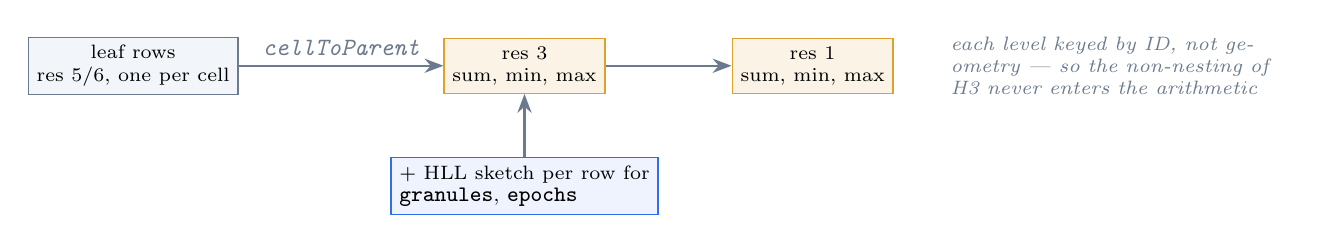
\begin{tikzpicture}[node distance=10mm]
  \node[bit, fill=panel] (leaf) {leaf rows\\\scriptsize res 5/6, one per cell};
  \node[bit, right=26mm of leaf, fill=metagold!12, draw=metagold] (r3) {res 3\\\scriptsize sum, min, max};
  \node[bit, right=16mm of r3, fill=metagold!12, draw=metagold] (r1) {res 1\\\scriptsize sum, min, max};
  \node[bit, below=8mm of r3, fill=idxblue!8, draw=idxblue, align=left] (hll)
    {\scriptsize + HLL sketch per row for\\\scriptsize \col{granules}, \col{epochs}};
  \draw[flow] (leaf) -- node[above, note] {\code{cellToParent}} (r3);
  \draw[flow] (r3) -- (r1);
  \draw[flow] (hll) -- (r3);
  \node[note, right=6mm of r1, text width=42mm] {each level keyed by ID, not geometry --- so the non-nesting
    of H3 never enters the arithmetic};
\end{tikzpicture}
\end{center}

\section{Adding time to the index}
\label{sec:time}

\emph{This section is speculative: a design sketch, not a description of what is built.}

\paragraph{The lede.} Sub-granule time is worth almost nothing, and the interesting work is all at the other
end. An ATL06 granule is one RGT quarter-orbit --- a few minutes of flight --- and the part of it inside one
res-5 cell is a few seconds. A time predicate finer than a granule therefore almost never eliminates a row
that the \emph{spatial} predicate has not already eliminated. What is missing is not resolution, it is
\emph{status}: time is a display field derived on the way out, not a predicate pushed into the scan, and it
is derived four different ways for four missions.

\paragraph{What already exists.} More than it looks like:

\begin{center}\small
\begin{tabular}{@{}llp{74mm}@{}}
\toprule
\textbf{Where} & \textbf{Grain} & \textbf{Form} \\
\midrule
granule name (ATL0x) & second   & \code{ATL06\_\underline{YYYYMMDDHHMMSS}\_\dots} --- parsed, no I/O \\
\col{gdate} (GLAS, ICESSN) & day & an index column, on every row \\
\col{cycle}, \col{rgt} (ATL0x) & 91-day repeat & index columns; the natural bucket for a repeat-track query \\
\col{ym} in \code{manifest.parquet} & month & \emph{already} the third of the \code{DISTINCT} triple \\
\col{delta\_time} & per segment & addressed by the chunk map, decoded only if fetched \\
\col{t} in the lake & millisecond & \code{timestamp[ms]}, per point \\
\bottomrule
\end{tabular}
\end{center}

\noindent
So a spatio-temporal query is already answerable end to end from the manifest, at granule grain --- but the
planner does it by intersecting cells first and filtering granule \emph{names} afterwards, in Python, after
the whole spatial result has been materialised.

\begin{center}
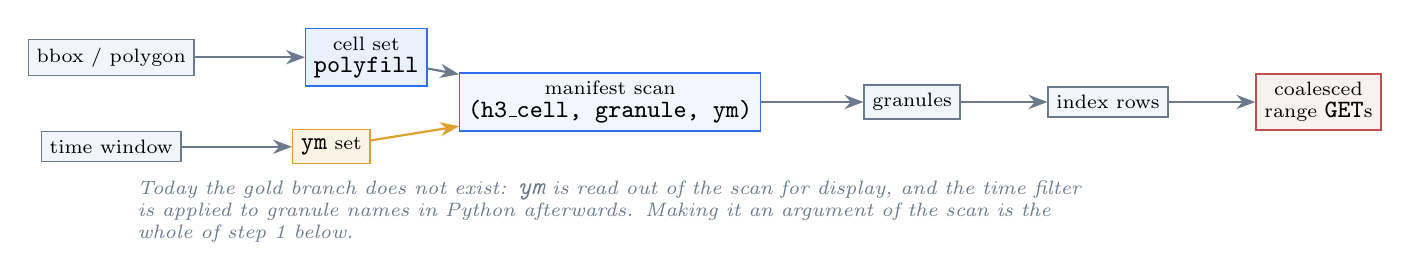
\begin{tikzpicture}[node distance=6mm, font=\footnotesize]
  \node[bit, fill=panel, align=center] (bbox) {bbox / polygon};
  \node[bit, below=7mm of bbox, fill=panel, align=center] (win) {time window};
  \node[bit, right=14mm of bbox, fill=idxblue!10, draw=idxblue] (cells) {cell set\\\scriptsize \code{polyfill}};
  \node[bit, right=14mm of win, fill=metagold!12, draw=metagold] (ym) {\code{ym} set};
  \node[bit, right=14mm of $(cells)!0.5!(ym)$, fill=idxblue!6, draw=idxblue, align=center] (scan)
    {manifest scan\\\scriptsize \code{(h3\_cell, granule, ym)}};
  \node[bit, right=13mm of scan, fill=panel] (gran) {granules};
  \node[bit, right=11mm of gran, fill=panel] (rows) {index rows};
  \node[bit, right=11mm of rows, fill=nasared!8, draw=nasared] (get) {coalesced\\range \code{GET}s};
  \draw[flow] (bbox) -- (cells);
  \draw[flow] (win) -- (ym);
  \draw[flow] (cells) -- (scan);
  \draw[flow, draw=metagold] (ym) -- (scan);
  \draw[flow] (scan) -- (gran); \draw[flow] (gran) -- (rows); \draw[flow] (rows) -- (get);
  \node[note, below=5mm of scan.south, text width=120mm, anchor=north]
    {Today the gold branch does not exist: \code{ym} is read out of the scan for display, and the time filter
     is applied to granule names in Python afterwards. Making it an argument of the scan is the whole of
     step 1 below.};
\end{tikzpicture}
\end{center}

\paragraph{Step 1 --- make \code{ym} a predicate, and partition the manifest by it.}
Push \code{ym BETWEEN} into the manifest scan, and write the rollup Hive-partitioned:
\code{\_coverage/ym=2019-03/part.parquet}, one \code{COPY \dots\ PARTITION\_BY (ym)} instead of one file.
A time predicate then becomes directory pruning and the spatial one stays row-group pruning inside each part.
This is the cheapest real win and it costs one line of the rebuild. The tradeoff to state plainly: a manifest
sorted or partitioned by time gives up the cell locality a spatial-only scan enjoys. Partitioning rather than
sorting is the compromise --- coarse pruning on time, order preserved on cell within each partition.

\paragraph{Step 2 --- one cross-mission space--time table.}
``Who observed this cell in 2019, from any mission?'' means four manifest scans with four different date
conventions today. A single \code{space\_time(mission, h3\_cell, ym, granules, n\_rows)} table in
\code{meta.duckdb}, produced by the same rollup pass, makes it one scan and normalises the date derivation in
exactly one place. It is also the natural home for the elevation time-series work, which currently
re-discovers coincident cells per query. Size is modest: the \code{DISTINCT (mission, cell, ym)} rollup drops
the granule dimension that makes the ATL06 manifest 2.3\,M rows.

\paragraph{Step 3 --- a time bucket in the key, only if the leaf count explodes.}
Same argument as \S\ref{sec:h3}: do not materialise a hierarchy while the leaf \code{GROUP BY} is free. If it
stops being free, the key becomes \((\text{h3\_cell},\ \text{bucket})\) --- \col{cycle} for ICESat-2, month
for the rest --- and the real question is the sort order, since neither cell-major nor time-major dominates.
The usual answer is a Z-order interleave of the two; the usual trap is assuming H3 IDs are spatially
contiguous under integer order. They are not: an H3 ID packs a base-cell number and then a digit sequence, so
integer order gives good locality \emph{within} one of the 122 base cells and none across them. Interleaving
\code{cellToParent(c,3)} with the time bucket is far better behaved than interleaving the raw 64-bit ID.

\paragraph{What I would not build.} \col{t\_min}/\col{t\_max} on the index row. Two doubles per row is nothing
in bytes, but populating them forces the builder to decode \col{delta\_time} for every chunk --- it currently
decodes only \col{latitude} and \col{longitude} --- and it buys a predicate the granule date already answers
to within a few minutes.

\paragraph{What would overturn this.} A collection whose granules span a long time: IceBridge campaign files,
or any future gridded or seasonally-aggregated product. For those the granule date is a bad proxy and
sub-granule time starts to earn its cost. If such a collection is added, revisit step 3 before step 1.

\section{Invariants}

Relied on throughout, and each violated at least once:

\begin{enumerate}\setlength{\itemsep}{2pt}
\item \textbf{Coverage is marked only after the file is on disk.} A crash loses cache, never truth.
\item \textbf{Index files land by rename.} Readers never see a torn Parquet, and the directory mtime is a
  sound change signal.
\item \textbf{All datasets of a beam share one chunk map.} \col{chunk\_index} is a single integer naming the
  same segment span in every dataset. The builder checks chunk length and chunk count against
  \col{latitude} (ATL06) or \col{h\_ph} (ATL03) and fails the build rather than assuming it.
\item \textbf{A lake file is written at the collection's own index resolution}, never at the planner's, so a
  partial cell is impossible by construction.
\item \textbf{Files are the source of truth for bytes and rows}; the metadata database is a cache of that
  truth, gated on a directory mtime, never the other way round.
\item \textbf{\code{coverage\_cells} is a superset of the materialised set}, by design. Counting files from
  it over-counts by $\approx 4\%$.
\end{enumerate}

\end{document}
